\section{Problem 6}\label{prob6}

To construct a BFS spanning tree, we use an algorithm similar to the one described in Problem \ref{prob3}, but with modified message types and handling rules to ensure the BFS property rather than an arbitrary spanning tree.

\subsection{Node Data Structure}
Each node in the network maintains the following information:
\begin{itemize}
    \item \textbf{Parent:} Initially set to \texttt{null}. (The node's parent in the BFS spanning tree.)
    \item \textbf{Children:} Initially an empty list. (The node's children in the BFS spanning tree.)
    \item \textbf{Forward Count:} Initially \texttt{0}. (Number of neighbors to which the node sent an \texttt{ASK}/\texttt{JOIN} message.)
    \item \textbf{Reply Count:} Initially \texttt{0}. (Number of replies received by the node.)
    \item \textbf{Level:} Initially \texttt{0}. (The node's level in the BFS spanning tree.)
    \item \textbf{New Node Found:} Initially \texttt{false}. (Flag indicating if a new node was added to the subtree rooted at the node during a phase.)
\end{itemize}

\subsection{Message Types}
The protocol utilizes the following message types:
\begin{itemize}
    \item \texttt{JOIN(LEVEL)}: Sent by the root to initiate the expansion to level \texttt{LEVEL}.
    \item \texttt{ASK(LEVEL)}: Sent by a node at level \texttt{LEVEL-1} to its neighbors asking them to join level \texttt{LEVEL}.
    \item \texttt{ACK}: Acknowledgment message sent by a node to its parent when it agrees to join the tree.
    \item \texttt{NACK}: Negative acknowledgment message sent by a node when it is already part of the tree.
    \item \texttt{DONE(LEVEL,NEW\_NODE\_FOUND)}: Sent by a node to its parent to indicate completion of level \texttt{LEVEL} in its subtree. The \texttt{NEW\_NODE\_FOUND} field is set to \texttt{true} if at least one new node was added to the tree.
\end{itemize}

\subsection{Algorithm Description}
Let's say at any phase \( i \), the BFS spanning tree has been constructed up to level \( i \), and termination has been detected by the root for this level. We now describe the process of expanding the tree to level \( i+1 \).

\begin{figure}[h]
    \centering
    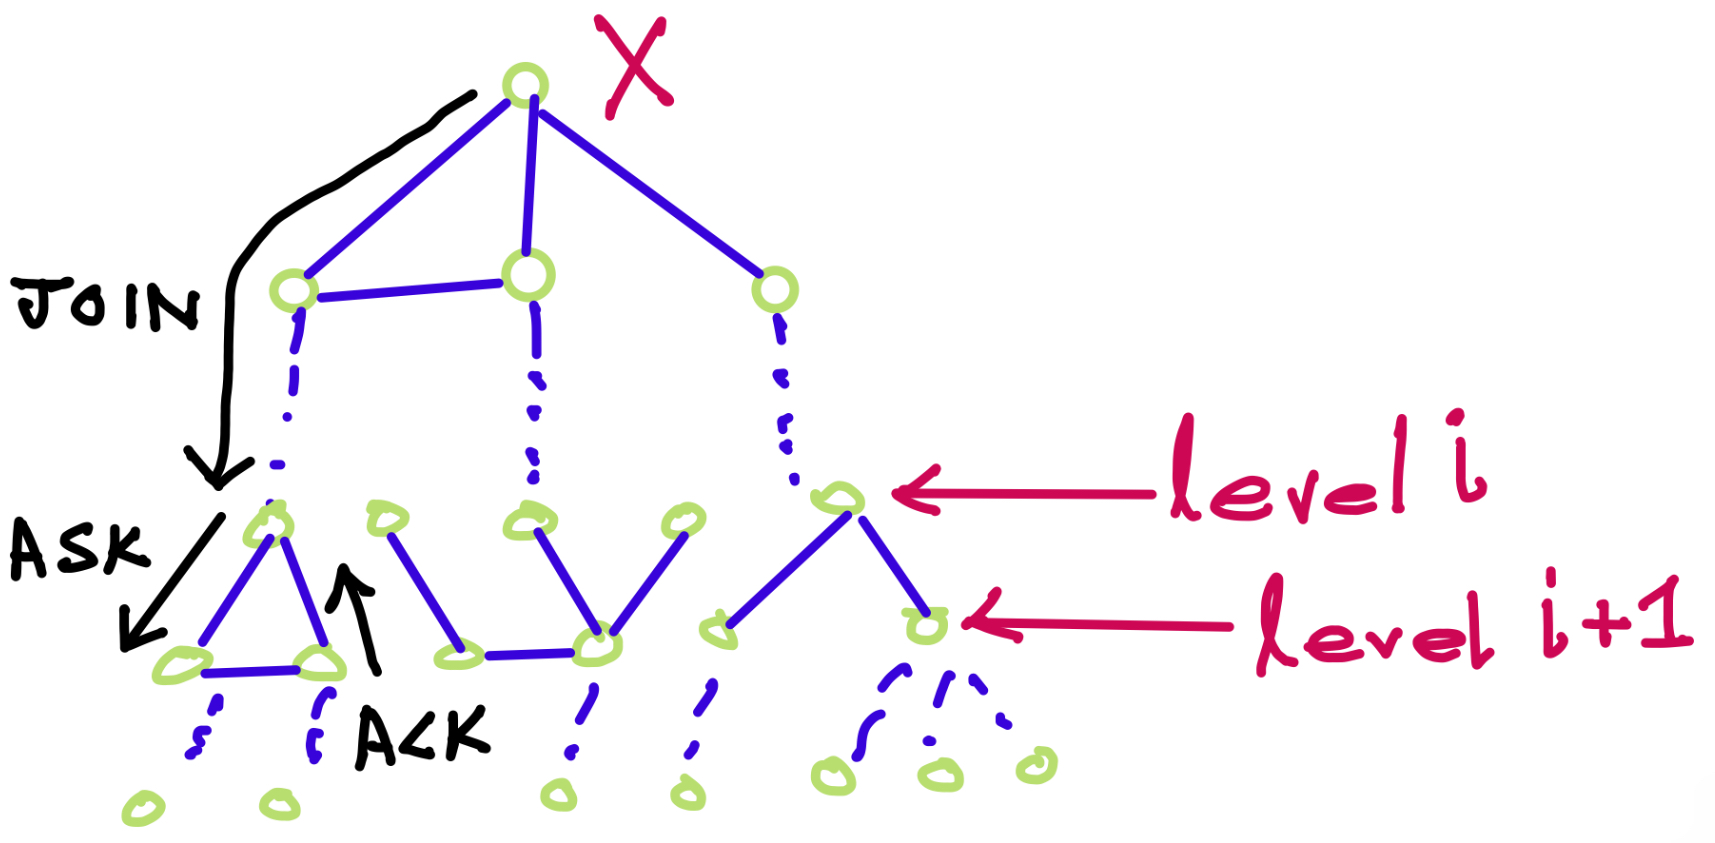
\includegraphics[width=0.5\textwidth]{IMG/Q6.jpeg}
    \caption{Expansion of the BFS Spanning Tree to Level \( i+1 \).}
    \label{fig:BFS}
\end{figure}

\subsubsection{Step 1: Sending JOIN Messages}
The root node initiates the process by sending a \texttt{JOIN(i+1)} message to all its \texttt{Children}. Any node \( u \) at level \( j \) (\( j < i \)) forwards this message to all its \texttt{Children}.

\subsubsection{Step 2: ASK and ACK/NACK Exchange}
When a node at level \( i \) receives \texttt{JOIN(i+1)}, it sends an \texttt{ASK(i+1)} message to all directly connected nodes except its \texttt{Parent}. It also sets:
\begin{itemize}
    \item \texttt{Forward Count} to the number of nodes to which it sent \texttt{ASK}.
    \item \texttt{Reply Count} to \texttt{0}.
\end{itemize}

Nodes that receive \texttt{ASK(i+1)} respond as follows:
\begin{itemize}
    \item If already part of the spanning tree, they send a \texttt{NACK}.
    \item If not part of the tree and receiving \texttt{ASK} for the first time:
    \begin{itemize}
        \item They send an \texttt{ACK}.
        \item They mark the sender as their \texttt{Parent} and set their \texttt{Level} to \( i+1 \).
    \end{itemize}
\end{itemize}

Nodes at level \( i \) collect \texttt{ACK} and \texttt{NACK} responses, updating:
\begin{itemize}
    \item \textbf{Children:} Nodes from which they receive \texttt{ACK}.
    \item \textbf{Reply Count:} Increments for every received \texttt{ACK} or \texttt{NACK}.
\end{itemize}

\subsubsection{Step 3: Propagating DONE Messages}
Once a node at level \( i \) has received replies from all nodes it sent \texttt{ASK} to (\texttt{Forward Count} = \texttt{Reply Count}), it sends a \texttt{DONE(LEVEL,NEW\_NODE\_FOUND)} message to its \texttt{Parent}. Here, \texttt{NEW\_NODE\_FOUND} is:
\begin{itemize}
    \item \texttt{true} if at least one \texttt{ACK} was received.
    \item \texttt{false} otherwise.
\end{itemize}

Nodes at top levels \( j\) \((j < i \)) wait for \texttt{DONE} messages from all their \texttt{Children} before forwarding the \texttt{DONE} message to their own \texttt{Parent}. The \texttt{NEW\_NODE\_FOUND} field is set to \texttt{true} if at least one child reported \texttt{NEW\_NODE\_FOUND = true}.

\subsubsection{Step 4: Root Detection of Termination}
The root node \(X\) receives \texttt{DONE} messages from all its \texttt{Children}. If any contain \texttt{NEW\_NODE\_FOUND = true}, it proceeds to phase \( i+2 \). Otherwise, the algorithm terminates, completing the BFS spanning tree construction.

This process can be repeated until the root detects that no new nodes were added to the tree in the last phase, signaling the completion of the BFS spanning tree.

\subsection{Message Handling Rules}

\subsubsection{Handling a \texttt{JOIN} Message}
When a node receives a \texttt{JOIN(i)} message:
\begin{itemize}
    \item If the node is at level \( i - 1 \), it sends an \texttt{ASK(i)} message to all its neighbors except the \texttt{Parent} and sets \texttt{New Node Found} to \texttt{false}. It also set the \texttt{Forward Count} to the number of neighbors to which it sent the message and \texttt{Reply Count} to \texttt{0}. (Nodes that are leaves in the current treen send \texttt{ASK} messages to all their neighbors asking them to join level \( i \).)
    \item If the node is at level \( j < i - 1 \), it forwards the message to all its \texttt{Children} and sets \texttt{Reply Count} to \texttt{0}. (Nodes that are not leaves in the current tree forward the \texttt{JOIN} message to their children.)
\end{itemize}

\subsubsection{Handling an \texttt{ASK} Message}
Upon receiving an \texttt{ASK(i)} message:
\begin{itemize}
    \item If the \texttt{Parent} field is not \texttt{null}, reply with a \texttt{NACK} message. (The node is already part of the BFS spanning tree.)
    \item Otherwise, reply with an \texttt{ACK} message, set the \texttt{Parent} field to the sender, and \texttt{Level} to \( i \). (The node joins the BFS spanning tree at level \( i \).)
\end{itemize}

\subsubsection{Handling an \texttt{ACK} Message}
Upon receiving an \texttt{ACK} message:
\begin{itemize}
    \item Add the sender to the \texttt{Children} list. (The sender is now a child of the node.)
    \item Increment the \texttt{Reply Count}. (The node has received a reply.)
    \item If \texttt{Reply Count} = \texttt{Forward Count}, send a \texttt{DONE(Level,true)} message to the \texttt{Parent}. (All replies have been received from the neighbors.)
\end{itemize}

\subsubsection{Handling a \texttt{NACK} Message}
Upon receiving a \texttt{NACK} message:
\begin{itemize}
    \item Increment the \texttt{Reply Count}. (The node has received a reply.)
    \item If \texttt{Reply Count} = \texttt{Forward Count}, check if the \texttt{Children} list is empty. If so, send a \texttt{DONE(level,false)} message to the \texttt{Parent}. Otherwise, send a \texttt{DONE(level,true)} message to the \texttt{Parent}. (All replies have been received from the neighbors. If no new nodes were explored, the \texttt{NEW\_NODE\_FOUND} field is set to \texttt{false}.)
\end{itemize}

\subsubsection{Handling a \texttt{DONE} Message}
Upon receiving a \texttt{DONE(i,NEW\_NODE\_FOUND)} message:
\begin{itemize}
    \item Increment the \texttt{Reply Count}. (The node has received a \texttt{DONE} message from a child indicating BFS tree construction up to level \( i \) in the child's subtree.)
    \item Set \texttt{New Node Found} to \( \texttt{New Node Found} \vee \texttt{NEW\_NODE\_FOUND} \). (Update the \texttt{New Node Found} flag based on the child's message.)
    \item If \texttt{Reply Count} = \texttt{Forward Count}, send a \texttt{DONE(i,New Node Found)} message to the \texttt{Parent}. (All replies have been received from the children. Send a message to the parent indicating completion of level \( i \) in the subtree.)
\end{itemize}


\subsection{Initialization and Termination}
The root node \( X \) initiates the BFS spanning tree construction by sending a \texttt{JOIN(1)} message to all its \texttt{Children}. It also sets itself as the root of the tree by setting its \texttt{Parent} field to \(X\) and \texttt{Level} to \(0\).

For each phase \( i \), the root sends a \texttt{JOIN(i)} message to all its \texttt{Children} and waits for \texttt{DONE(i, NEW\_NODE\_FOUND)} messages from all of them. If at least one \texttt{DONE} message contains \texttt{NEW\_NODE\_FOUND = true}, the process continues to phase \( i+1 \). Otherwise, the algorithm terminates, signaling the completion of the BFS spanning tree.

\subsection{Message Complexity}
Let \( N \) represent the number of nodes in the network, \( M \) the number of edges, and \( D \) the diameter.

The number of rounds is bounded by the network's diameter. For each edge \( (u, v) \), the \texttt{ASK} and \texttt{ACK}/\texttt{NACK} messages are exchanged at most twice, resulting in a maximum of 4 messages per edge, leading to \( 4 \times M \) messages in total.

In each round, \texttt{JOIN} and \texttt{DONE} messages are exchanged across the tree edges, with a total of at most \( 2 \times (N-1) \) messages per round. Hence, the overall message complexity is:
\[
O(N \times D + M).
\]

